\chapter{Bayes Nets to Junction trees}

Figure~\ref{figure:bayes_net} is the Bayes Net for the Kalman Filter. The control vector, $\mathbf{u}_t = \mathbf{u}$, may be neglected in most cases as it is a constant. Each node is a Gaussian CPD with:

\documentclass[tikz]{standalone}
\usepackage{amsfonts}
\usepackage{amsmath}
\usepackage{amssymb}
\usepackage{tikz}
\begin{document}

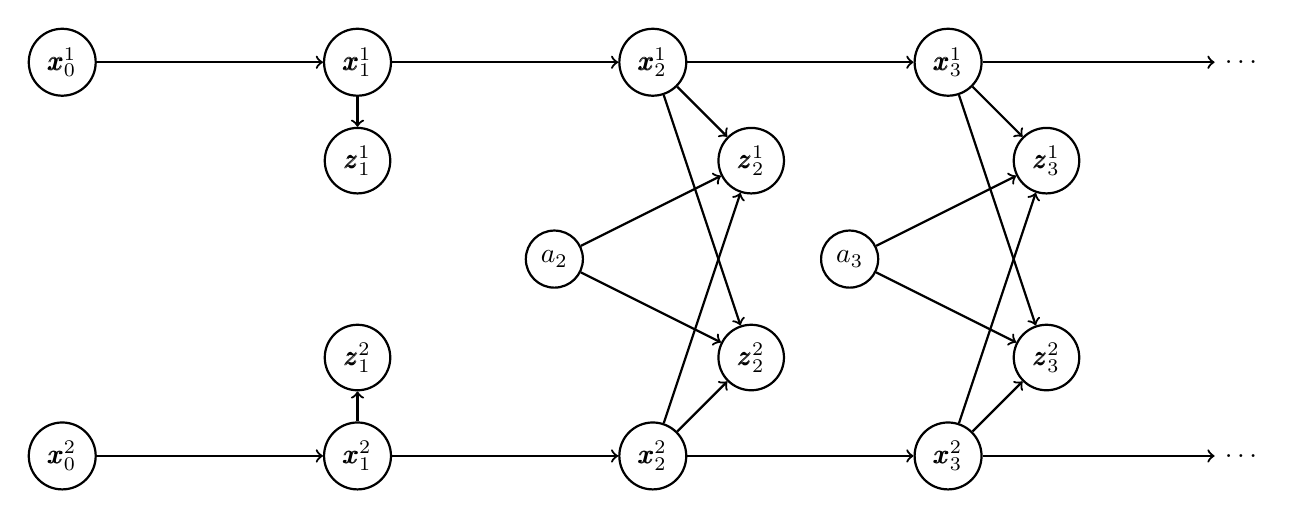
\begin{tikzpicture}

\begin{scope}[every node/.style={circle,thick,draw}]
	%Frame 1
	\node (x_0^1) at (-3.75, 0) {$\pmb{x}_{0}^{1}$};
	\node (x_0^2) at (-3.75, -5) {$\pmb{x}_{0}^{2}$};
	
	%Frame 2
	\node (x_1^1) at (0, 0) {$\pmb{x}_{1}^{1}$};
	\node (z_1^1) at (0, -1.25) {$\pmb{z}_{1}^{1}$};
	
	\node (z_1^2) at (0, -3.75) {$\pmb{z}_{1}^{2}$};
	\node (x_1^2) at (0, -5) {$\pmb{x}_{1}^{2}$};
	
	%Frame 3
	\node (x_2^1) at (3.75, 0) {$\pmb{x}_{2}^{1}$};
	
	\node (a_2) at (2.5, -2.5) {$a_{2}$};
	\node (z_2^1) at (5, -1.25) {$\pmb{z}_{2}^{1}$};
	\node (z_2^2) at (5, -3.75) {$\pmb{z}_{2}^{2}$};
	
	\node (x_2^2) at (3.75, -5) {$\pmb{x}_{2}^{2}$};
	
	%Frame 4
	\node (x_3^1) at (7.5, 0) {$\pmb{x}_{3}^{1}$};
	
	\node (a_3) at (6.25, -2.5) {$a_{3}$};
	\node (z_3^1) at (8.75, -1.25) {$\pmb{z}_{3}^{1}$};
	\node (z_3^2) at (8.75, -3.75) {$\pmb{z}_{3}^{2}$};
	
	\node (x_3^2) at (7.5, -5) {$\pmb{x}_{3}^{2}$};
\end{scope}

\begin{scope}[style={thick,draw}]
	%Frame 5
    \node (xdot1) at (11.25, 0) {\dots};
    \node (xdot2) at (11.25, -5) {\dots};
\end{scope}

\begin{scope}[style={thick,draw}]
	%Frame 1
	\path [->] (x_0^1) edge node {} (x_1^1);
	\path [->] (x_0^2) edge node {} (x_1^2);
	
	%Frame 2
	\path [->] (x_1^1) edge node {} (x_2^1);
	\path [->] (x_1^1) edge node {} (z_1^1);
	
	\path [->] (x_1^2) edge node {} (z_1^2);
	\path [->] (x_1^2) edge node {} (x_2^2);

	%Frame 3
	\path [->] (x_2^1) edge node {} (x_3^1);
	\path [->] (x_2^1) edge node {} (z_2^1);
	\path [->] (x_2^1) edge node {} (z_2^2);
	
	\path [->] (a_2) edge node {} (z_2^1);
	\path [->] (a_2) edge node {} (z_2^2);
	
	\path [->] (x_2^2) edge node {} (x_3^2);
	\path [->] (x_2^2) edge node {} (z_2^1);
	\path [->] (x_2^2) edge node {} (z_2^2);
		
	%Frame 4
	\path [->] (x_3^1) edge node {} (xdot1);
	\path [->] (x_3^1) edge node {} (z_3^1);
	\path [->] (x_3^1) edge node {} (z_3^2);
	
	\path [->] (a_3) edge node {} (z_3^1);
	\path [->] (a_3) edge node {} (z_3^2);
	
	\path [->] (x_3^2) edge node {} (z_3^1);
	\path [->] (x_3^2) edge node {} (z_3^2);
	\path [->] (x_3^2) edge node {} (xdot2);
\end{scope}

\end{tikzpicture}

\end{document}

\begin{eqnarray}
p(\mathbf{x}_t | \mathbf{x}_{t-1}) &=& \mathcal{N}(\mathbf{x}_{t} | A \mathbf{x}_{t-1} + B\mathbf{u}, R) \label{eqn:transition} \\
p(\mathbf{z}_t | \mathbf{x}_{t}) &=& \mathcal{N}(\mathbf{z}_{t} | C\mathbf{x}_{t}, Q) \label{eqn:measurement} \\
p(\mathbf{x}_{0}) &=& \mathcal{N}(\mathbf{x}_{0}| \mathbf{\mu}_{0}, \Sigma_{0}) \label{eqn:belief}
\end{eqnarray}

Figure~\ref{figure:junction_tree} is the network's equivalent Junction Tree. This Junction Tree was created following the procedure given in the PGM: Week 5 notes. Moralization and triangulation shouldn't affect the structure and the induced graph should be an undirected equivalent of the Bayes Net. The maximal cliques will be allocated a single potential, corresponding to their CPDs in Equations~\ref{eqn:transition} and ~\ref{eqn:measurement}.

\section{Message passing: Integral-Product algorithm}

I assume that the discrete message passing algorithm is replaced with:

\begin{eqnarray}
\delta_{\phi_{\mathbf{x}_{t}} \rightarrow \phi_{\mathbf{x}_{t+1}}}(\mathbf{x}_{i}) &=& \int \phi_{\mathbf{x}_{t}}(\mathbf{x}_{t}, \mathbf{x}_{t-1}) \delta_{\mathbf{z}_{t} \rightarrow \mathbf{x}_{t}} (\mathbf{x}_{t}) \delta_{\mathbf{x}_{t} \rightarrow \mathbf{x}_{t+1}} (\mathbf{x}_{t-1}) d\mathbf{x}_{t-1} 
\end{eqnarray}

I assme the idea is to use canonical form to ease the marginalization.
\begin{figure}
\centering
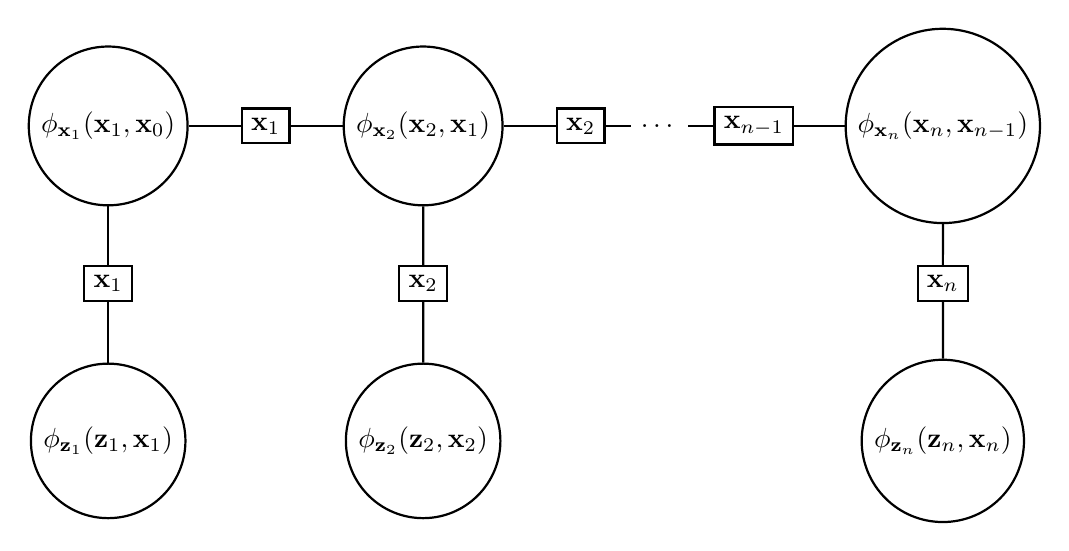
\begin{tikzpicture}[scale=0.80]
\begin{scope}[every node/.style={circle,thick,draw}]
    \node (x1) at (0, 0) {$\phi_{\mathbf{x}_1} (\mathbf{x}_{1}, \mathbf{x}_{0})$};
    \node (z1) at (0, -5) {$\phi_{\mathbf{z}_1} (\mathbf{z}_{1}, \mathbf{x}_{1})$};

    \node (x2) at (5, 0) {$\phi_{\mathbf{x}_2} (\mathbf{x}_{2}, \mathbf{x}_{1})$};
    \node (z2) at (5, -5) {$\phi_{\mathbf{z}_2} (\mathbf{z}_{2}, \mathbf{x}_{2})$};
    
    \node (xn) at (13.25, 0) {$\phi_{\mathbf{x}_n} (\mathbf{x}_{n}, \mathbf{x}_{n-1})$};
    \node (zn) at (13.25, -5) {$\phi_{\mathbf{z}_n} (\mathbf{z}_{n}, \mathbf{x}_{n})$};

\end{scope}

\begin{scope}[every node/.style={thick,draw}]
    \node (sz1) at (0, -2.5) {$\mathbf{x}_{1}$};
    \node (sx1) at (2.5, 0) {$\mathbf{x}_{1}$};
    
    \node (sz2) at (5, -2.5) {$\mathbf{x}_{2}$};
    \node (sx2) at (7.5, 0) {$\mathbf{x}_{2}$};
    
    \node (sxn) at (10.25,0) {$\mathbf{x}_{n-1}$};
    \node (szn) at (13.25, -2.5) {$\mathbf{x}_{n}$};
\end{scope}

\begin{scope}[style={thick,draw}]
    \node (xdot1) at (8.75,0) {\dots};
\end{scope}


\begin{scope}[style={thick,draw}]
	\path [-] (x1) edge node {} (sz1);
	\path [-] (sz1) edge node {} (z1);
	\path [-] (x1) edge node {} (sx1);
	\path [-] (sx1) edge node {} (x2);
	
	\path [-] (x2) edge node {} (sz2);
	\path [-] (sz2) edge node {} (z2);
	\path [-] (x2) edge node {} (sx2);
	\path [-] (sx2) edge node {} (xdot1);

	\path [-] (xdot1) edge node {} (sxn);	
	\path [-] (sxn) edge node {} (xn);
	\path [-] (xn) edge node {} (szn);	
	\path [-] (szn) edge node {} (zn);
	
\end{scope}

\end{tikzpicture}

\caption[Equivalent Junction Tree for a Kalman Filter.]{The junction tree  resulting  from the Bayes Net in Figure~\ref{figure:bayes_net}.}
\label{figure:junction_tree}
\end{figure}